\documentclass[../mathNotesPreamble]{subfiles}

\providecommand{\relscalefact}{1.4}
\begin{document}
\relscale{\relscalefact}
  \section{1.5: Solutions of Systems of Linear Equations}
  \begin{center}
    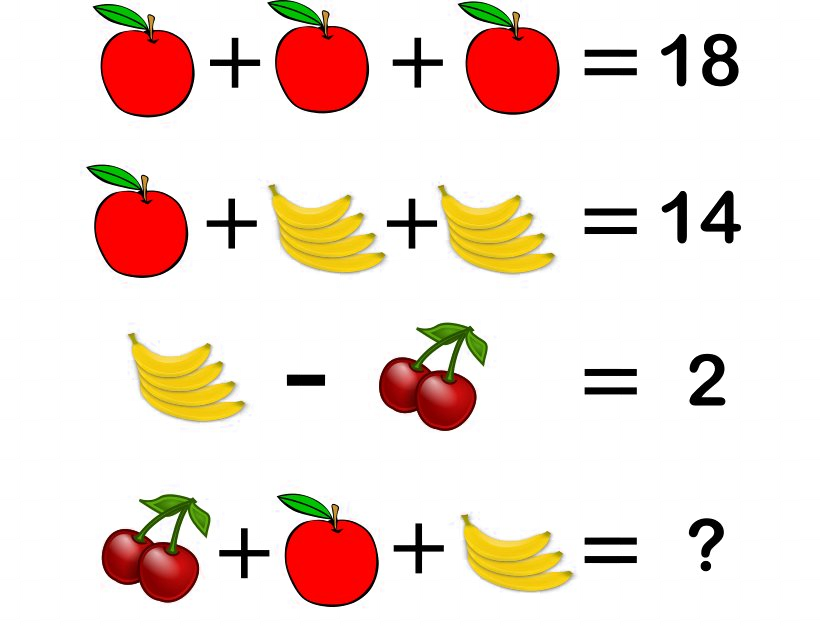
\includegraphics[width=0.65\linewidth]{images/fruit_math_puzzle}
  \end{center}
  \vspace*{\stretch{1}}

  \begin{defn*}
    A \textbf{system of equations} is $2$ (or more) equations. The ordered pairs $(x,y)$ that satisfies \emph{all} equations in the system are the \textbf{solutions} of the system.
  \end{defn*}
  \vspace*{\stretch{1}}

  When solving a system of linear equations, there are three possible outcomes:
  \begin{center}
    \begin{minipage}{0.5\linewidth}
      \begin{enumerate}
        \item No solution (\emph{Inconsistent}),
        \item Exactly one solution,
        \item Infinitely many solutions (\emph{Dependent}).
      \end{enumerate}
    \end{minipage}
  \end{center}
  \pagebreak

  \begin{ex*}
    Use graphing to find the solutions to the following systems
  \end{ex*}
  \noindent
    \begin{minipage}{0.45\linewidth}
      \begin{alignat*}{3}
%        r&l&r&l&r\\
        2x&\,-\,&6y&=&-6\\
        -x&\,+&\,3y&=&\,-3
      \end{alignat*}
    \end{minipage}%
%    \hspace*{\stretch{1}}
    \begin{minipage}{0.45\linewidth}
      \begin{flushright}
        \begin{tikzpicture}[scale=0.8, declare function={
          f(\x)=1*\x/3+1;
          g(\x)=1*\x/3-1;}]
          \begin{axis}[
            axis lines=center,
            axis line style={black,->},
%            minor x tick num=1,
            minor y tick num=1,
            ticklabel style={font=\footnotesize,inner sep=0.5pt,fill=white,opacity=1.0, text opacity=1},
            xlabel=$x$, xlabel style={at={(ticklabel* cs:1)},anchor=north west},
            ylabel=$y$, ylabel style={at={(ticklabel* cs:1)},anchor=south west},
            every axis plot/.append style={line width=0.95pt, color=lander_blue, samples=255}
            ]
            \addplot[<->] expression[domain=-3:5.5]{f(x)}
              node[pos=0.75, above left, xshift=15pt, black] {$2x-6y=-6$};
            \addplot[<->] expression[red, domain=-3:5.5]{g(x)}
              node[pos=0.4, below right, black] {$-x+3y=-3$};
          \end{axis}
        \end{tikzpicture}
      \end{flushright}
    \end{minipage}%
    \vspace*{\stretch{1}}

    \noindent
    \begin{minipage}{0.45\linewidth}
      \begin{alignat*}{3}
%        r&l&r&l&r\\
        4x&\,+\,&3y&=&11\\
        2x&\,-&\,5y&=&\,-1
      \end{alignat*}
    \end{minipage}%
%    \hspace*{\stretch{1}}
    \begin{minipage}{0.45\linewidth}
      \begin{flushright}
        \begin{tikzpicture}[scale=0.8, declare function={
          f(\x)=-4*\x/3+11/3;
          g(\x)=2*\x/5+1/5;}]
          \begin{axis}[
            axis lines=center,
            axis line style={black,->},
%            minor x tick num=1,
            minor y tick num=1,
            ticklabel style={font=\footnotesize,inner sep=0.5pt,fill=white,opacity=1.0, text opacity=1},
            xlabel=$x$, xlabel style={at={(ticklabel* cs:1)},anchor=north west},
            ylabel=$y$, ylabel style={at={(ticklabel* cs:1)},anchor=south west},
            every axis plot/.append style={line width=0.95pt, color=lander_blue, samples=255}
            ]
            \addplot[<->] expression[domain=-1.5:5.5]{f(x)}
              node[pos=0.875, below left, black] {$4x+3y=11$};
            \addplot[<->] expression[red, domain=-1.5:5.5]{g(x)}
              node[pos=0.975, above left, black] {$2x-5y=-1$};
          \end{axis}
        \end{tikzpicture}
      \end{flushright}
    \end{minipage}%
    \vspace*{\stretch{1}}

    \noindent
    \begin{minipage}{0.45\linewidth}
      \begin{alignat*}{3}
%        r&l&r&l&r\\
        -4x&\,+\,&3y&=&-2\\
        8x&\,-&\,6y&=&\,4
      \end{alignat*}
    \end{minipage}%
%    \hspace*{\stretch{1}}
    \begin{minipage}{0.45\linewidth}
      \begin{flushright}
        \begin{tikzpicture}[scale=0.8, declare function={
          f(\x)=4*\x/3-2/3;
          g(\x)=4*\x/3-2/3;}]
          \begin{axis}[
            axis lines=center,
            axis line style={black,->},
%            minor x tick num=1,
            minor y tick num=1,
            ticklabel style={font=\footnotesize,inner sep=0.5pt,fill=white,opacity=1.0, text opacity=1},
            xlabel=$x$, xlabel style={at={(ticklabel* cs:1)},anchor=north west},
            ylabel=$y$, ylabel style={at={(ticklabel* cs:1)},anchor=south west},
            every axis plot/.append style={line width=0.95pt, color=lander_blue, samples=255}
            ]
            \addplot[<->] expression[domain=-1.5:5.5]{f(x)}
              node[pos=0.45, below right, black] {$-4x+3y=-2$};
            \addplot[<->,dashed] expression[red, domain=-1.5:5.5]{g(x)}
              node[pos=0.75, above left, black] {$8x-6y=4$};
          \end{axis}
        \end{tikzpicture}
      \end{flushright}
    \end{minipage}%

  \pagebreak
  \noindent
  \fbox{\parbox{0.9875\linewidth}{\textbf{Equivalent systems} result when
    \begin{enumerate}
      \item One expression is replaced by an equivalent expression.
      \item Two equations are interchanged.
      \item A multiple of one equation is added to another equation.
      \item An equation is multiplied by a nonzero constant.
    \end{enumerate}
  }}
  \vspace*{\stretch{1}}

  \noindent
  \fbox{\parbox{0.9875\linewidth}{\textbf{Substitution Method}
    \begin{ex*}
      Solve the system
      $\left \{ \begin{array}{*{3}{@{}r@{}l}}
%        r&l&r&l&r\\
        2x&\,+\,&3y&=&4\\
        x&\,-&\,2y&=&\,3
      \end{array}\right.$
    \end{ex*}
    \begin{minipage}[t]{0.475\linewidth}
      \begin{enumerate}
        \item Solve one equation for either one of the variables in terms of the other.
        \item Substitute this expression into the other equation to give the equation in one unknown.
        \item Solve this equation for the unknown.\\
        \item Substitute solution into the equation in Step 1.\\
        \item Check the solution $(x,y)$.
      \end{enumerate}
    \end{minipage}%
    \hspace*{\stretch{1}}
    \begin{minipage}[t]{0.45\linewidth}
      \addtolength{\jot}{15pt}
      \begin{align*}
        x&=2y+3\\
        2\parens{\textcolor{red}{2y+3}}+3y&=4\\[0.5\baselineskip]
        4y+6+3y&=4\\[-20pt]
        7y&=-2 \Rightarrow y=-\frac{2}{7}\\
        x&=2\parens{\textcolor{red}{-\frac{2}{7}}}+3 \Rightarrow x=\frac{17}{7}\\
      &\begin{array}{*{3}{@{}r@{}l}}
%        r&l&r&l&r\\
        2\parens{\textcolor{red}{\displaystyle\frac{17}{7}}}&\,+\,&3\parens{\textcolor{red}{-\displaystyle\frac{2}{7}}}&=&4\\[10pt]
        \parens{\textcolor{red}{\displaystyle\frac{17}{7}}}&\,-&\,2\parens{\textcolor{red}{-\displaystyle\frac{2}{7}}}&=&\,3
      \end{array}
    \end{align*}
    \end{minipage}%
    \vspace*{5pt}
  }}
  \pagebreak

  \begin{ex*}
    Use the substitution method to solve the system
      \begin{center}
        \begin{alignat}{3}
%          r&l&r&l&r\\
          4x&\,+\,&5y&=&18\\
          3x&\,-&\,9y&=&\,-12
        \end{alignat}
      \end{center}
  \end{ex*}
  \vspace*{\stretch{1}}
  \pagebreak

  \noindent
  \fbox{\parbox{0.9875\linewidth}{\textbf{Elimination Method}
    \begin{ex*}
      Solve the system
      $\left \{ \begin{array}{*{3}{@{}r@{}l}}
%        r&l&r&l&r\\
        2x&\,-\,&5y&=&4\\
        x&\,+&\,2y&=&\,3
      \end{array}\right.$
    \end{ex*}
    \begin{minipage}[t]{0.475\linewidth}
      \begin{enumerate}
        \item Multiply one or both equations by a nonzero number so the coefficients of one of the variables may cancel.
        \item Add or subtract the equations to eliminate one of the variables.
        \item Solve for the remaining variable.
        \item Substitute solution in one of the original equations and solve for the other variable.
        \item Check the solution $(x,y)$
      \end{enumerate}
    \end{minipage}%
    \hspace*{\stretch{1}}
    \begin{minipage}[t]{0.45\linewidth}
      \addtolength{\jot}{15pt}
      \begin{align*}
        &\Rightarrow \left \{ \begin{array}{*{3}{@{}r@{}l}}
%        r&l&r&l&r\\
        2x&\,-\,&5y&=&4\\
        -2x&\,-&\,4y&=&\,-6
      \end{array}\right.\\
      &\phantom{\Rightarrow}\hspace*{24pt}\textcolor{red}{0x}-9y=-2\\
      &\Rightarrow y=\frac{2}{9}\\
      & 2x-5\parens{\textcolor{red}{\frac{2}{9}}}=4
      \ \Rightarrow x=\frac{23}{9}\\
        &\begin{array}{*{3}{@{}r@{}l}}
%          r&l&r&l&r\\
          2\parens{\textcolor{red}{\displaystyle\frac{23}{9}}}&\,-\,&5\parens{\textcolor{red}{\displaystyle\frac{2}{9}}}&=&4\\[10pt]
          \parens{\textcolor{red}{\displaystyle\frac{23}{9}}}&\,+&\,2\parens{\textcolor{red}{\displaystyle\frac{2}{9}}}&=&\,3
      \end{array}
    \end{align*}
    \end{minipage}%
    \vspace*{5pt}
  }}
  \pagebreak

  \begin{ex*}
    Use the elimination method to solve the following systems:
  \end{ex*}
  \noindent
  \begin{minipage}{0.25\linewidth}
    \begin{alignat*}{3}
%      r&l&r&l&r\\
      2x&\,-\,&6y&=&-6\\
      -x&\,+&\,3y&=&\,-3
    \end{alignat*}
  \end{minipage}%
  \vspace*{\stretch{1}}

  \noindent
  \begin{minipage}{0.25\linewidth}
    \begin{alignat*}{3}
%      r&l&r&l&r\\
      4x&\,+\,&3y&=&11\\
      2x&\,-&\,5y&=&\,-1
    \end{alignat*}
  \end{minipage}%
  \vspace*{\stretch{1}}

  \noindent
  \begin{minipage}{0.25\linewidth}
    \begin{alignat*}{3}
%      r&l&r&l&r\\
      -4x&\,+\,&3y&=&-2\\
      8x&\,-&\,6y&=&\,4
    \end{alignat*}
  \end{minipage}
  \vspace*{\stretch{1}}
  \pagebreak

  \begin{ex*}
    A woman has \$500,000 invested in two rental properties. One yields an annual return of 10\% on her investment, and the other returns 12\% per year on her investment. Her total annual return from the two investments is \$53,000. Let $x$ represent the amount of the 10\% investment and $y$ represent the amount of the 12\% investment.
  \end{ex*}
  \begin{tasks}[after-item-skip=2.5\baselineskip, label=\textbullet](1)
    \task Write an equation that states that the sum of investments is \$500,000.
    \task What is the annual return on the 10\% investment? What about the 12\% investment?
    \task Write an equation that states the sum of the annual return is \$53,000.
    \task Solve these two equations simultaneously to find how much is invested in each property.
  \end{tasks}
  \vspace*{\stretch{1}}
  \pagebreak

  \begin{ex*}
    A nurse has two solutions that contain different concentrations of a certain medication. One is a 12.5\% concentration, and the other is a 5\% concentration. How many cubic centimeters of each should she mix to obtain 20 cubic centimeters of an 8\% concentration?
  \end{ex*}
  \pagebreak

  \begin{ex*}
    Using U.S. Bureau of Labor Statistics data for selected years from 1950 and projected to 2050, the number of men $M$ and women $W$ in the workforce (both in millions) can be modeled by the functions
      \[M(t)=0.591t+37.3 \hspace*{20pt}\textnormal{ and }\hspace*{20pt} W(t)=0.786t+13.1\]
    where $t$ is the number of years after 1940. Find the year these functions predict that there will be equal numbers of men and women in the U.S. workforce.
  \end{ex*}
  \begin{flushright}
    \begin{tikzpicture}[scale=1.0, declare function={
      M(\t)=0.591*\t+37.3;
      W(\t)=0.786*\t+13.1;}]
      \begin{axis}[
        axis lines=center,
        axis line style={black,->},
%        minor x tick num=1,
%        minor y tick num=1,
        enlargelimits={value=0.05, auto},
        ticklabel style={font=\footnotesize,inner sep=0.5pt,fill=white,opacity=1.0, text opacity=1},
        xlabel=$t$, xlabel style={at={(ticklabel* cs:1)},anchor=north west},
        % ylabel=$y$, ylabel style={at={(ticklabel* cs:1)},anchor=south west},
        every axis plot/.append style={line width=0.95pt, color=lander_blue, samples=255}
        ]
        \addplot[<->] expression[domain=0:200]{M(x)}
          node[pos=0.35, above left, black] {$M(t)$};
        \addplot[<->] expression[red,domain=0:200]{W(x)}
          node[pos=0.35, below right, black] {$W(t)$};
      \end{axis}
    \end{tikzpicture}
  \end{flushright}

  \pagebreak
\end{document}
